\documentclass[12pt,a4paper]{scrartcl}

\usepackage[T1]{fontenc}
\usepackage[utf8]{inputenc}
\usepackage[magyar]{babel}
\usepackage{lmodern}
%% Sets page size and margins
\usepackage[a4paper,top=3cm,bottom=2cm,left=3cm,right=3cm,marginparwidth=1.75cm]{geometry}

\usepackage{graphicx}
\usepackage{amsmath}
\usepackage{amsfonts}
\usepackage{amssymb}
\usepackage{bm}
\let\mathbf\bm

\usepackage{placeins}
\usepackage{subcaption}
\usepackage{epstopdf}
\usepackage{xcolor}
\usepackage[hidelinks,unicode]{hyperref}
\hypersetup{
    colorlinks,
    linkcolor={red!50!black},
    citecolor={blue!50!black},
    urlcolor={blue!80!black}
}

\usepackage{cleveref}

\title{Felületi feszültség\\{\small{7. tétel}}}
\author{Tüzes Dániel}
\date{\today}
\begin{document}
\maketitle

\section{Felületi feszültség}

\footnotesize
\paragraph{Demonstráció} Egy vékony pengét a víz felszínére teszünk. A penge sűrűsége nagyobb, mint a vízé, alakja nem konkáv, így a víz nem tud akkora felhajtóerőt kifejteni rá, ami meggátolhatná az elsüllyedésben. Mégis, a víz felszínére óvatosan ráhelyezett penge nem merül el a vízben. Ha a víz alá nyomjuk, akkor már elsüllyed.

A víz felszínén úszó, lemezből készült hajókának a végére étert cseppentünk, akkor a hajó elindul előre. Szappan bekenve a végét hasonló jelenséget tapasztalunk.

Egy pohár tetejét egy rétegben egy hálóval fedjük be, pl.\ gézlappal. A poharat megtöltjük vízzel. Ha a poharat ügyesen megfordítjuk, akkor a víz nem jön ki a pohárból, annak ellenére, hogy a hálón könnyen át tudna folyni. Ha a hálóhoz hozzáérünk, a folyadék kifolyik.
\normalsize

Megfigyelés: Ha egy téglalap drótkeretén szappanhártya feszül, és a téglalap egyik oldala szabadon mozoghat, akkor a szappanhártya a szabadon mozgó oldalt elmozdítja úgy, hogy a téglalap területe csökkenjen. Ahhoz, hogy a szabad oldal ne mozduljon el, erőt kell kifejteni, aminek a nagysága függ az anyagi minőségtől, és a keretben lévő szál hosszától.
\[F = 2\alpha  \cdot l\]
A definícióban szereplő $2$-es nem véletlen, bár egyelőre csak definíció kérdése a léte. Ebben a képletben $\alpha$-t felületi feszültségnek nevezzük, és a  mértékegysége $\text{ N}/\text{m}$.

\begin{figure}[htbp]
	\begin{center}
		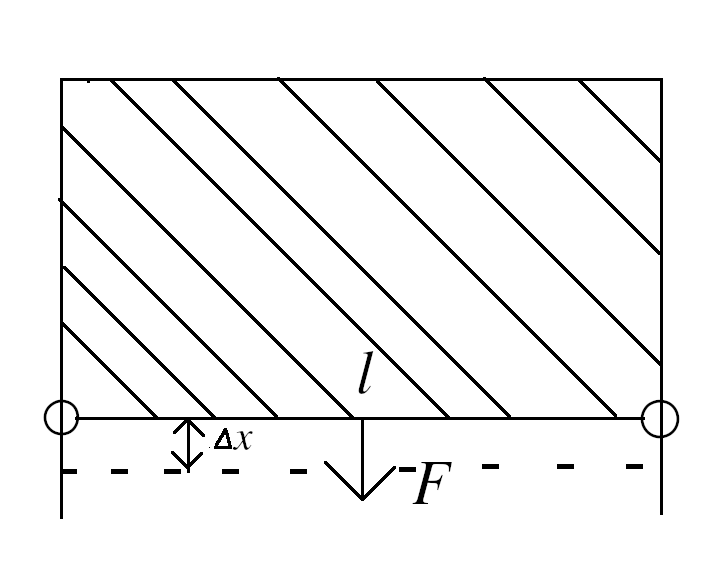
\includegraphics[width=0.4\textwidth]{tetel7.png}
		\caption{A fémkeret, benne a hártyával. $F$ erővel $\Delta x$ távolsággal kihúzzuk, így a felület $\Delta A =  2l \cdot \Delta x$-nyit megnő. A kettes szorzó azt fejezi ki, hogy a felületnek két oldala van.}
	\end{center}
\end{figure}

A felületi feszültségnek egy másik értelmezését is megadhatjuk, ha feltesszük a kérdést, hogy mennyivel változik meg a hártya által tárolt energia, miközben megváltoztatom a hártya nagyságát? Ehhez keret oldalát mozdítsuk el egy $\Delta x$ távolsággal! A mozgatás során erő nem változik, így a végzett munka
\[\Delta W = F \cdot \Delta x = \alpha 2l \cdot \Delta x = \alpha  \cdot \Delta A.\]

A felületi feszültségre ebből a képletből adódik az alábbi alak:
\[\alpha  = \frac{{dW}}{{dA}}.\]

Ha a felületi feszültség definíciójának ezt tekintjük, akkor ebben már nincs 2-es, és amúgy pontosan ezért lett korábban az erő kifejezésében egy 2-es beleépítve, hogy ebben már ne legyen. A felületi feszültség tehát megadja, hogy mennyivel nő meg egy felület energiája, ha a felszínét megváltoztatom.

A felületi feszültség minden határfelületen fellép. Energetikai szempontból a minimális határfelületű alakzatok a legkedvezőbbek, ezért a hártya mindig abba az alakba igyekszik beállni. 

\footnotesize
\paragraph{Demonstráció} Egy 2D-s keret esetén, ha a keret alakja téglalap, triviális, hogy mi a minimális felület, ha az egyik oldalt szabadon mozgathatjuk. Nem triviális azonban, ha a peremfeltételeket 3D-ben írjuk fel. A megoldásokat egyből láthatjuk, amennyiben a peremfeltételeket drótból kihajlítjuk és szappanos vízbe tesszük, majd kivesszük. Nem csak a hártya szélére írhatunk fel feltételeket, hanem felírhatunk bizonyos kényszereket is, mint pl.\ hogy valamilyen tartományra a térfogat legyen (hozzávetőleg) állandó.
\normalsize

Mi a felületi feszültség mikroszkopikus forrása? Tekintsünk egy folyadékot, és az annak a belsejében lévő molekulákat. Ezeket a molekulákat a többi minden oldalról körülveszi, és így vannak egyensúlyban. A felszínen lévő molekulák is egyensúlyban vannak, pedig azokra a többi molekula csak oldalsó, illetve a folyadék belsejéből származó erő tud hatni. A felületi feszültség azt mondja, hogy ahhoz, hogy olyan molekulából, amire mindenhonnan hat erő, olyan helyre mozdítsam, amire 1 oldalról már nem hat erő, munkát kell végezzek.

\footnotesize
\paragraph{Storytime} A felületi feszültség egy egyetemes jelenség a fizikában. Nem csak szappanhártyáknál, víznél, és úgy általában véve, folyadékoknál, de minden közeghatáron fellép. Ilyenek például összeolvadt szemcsék határa ugyanazon anyagon belül (cink kristályszemcsék a színtiszta cinkben), vagy a szilárd ötvözetekben az egyes alkotók alkotta kiválások határa is. Ez utóbbira példa az acél, ami vas és szén ötvözete. Az acélban a szén kiválásokat képez, és a szén-vas felületen a felületi feszültség megváltoztatja az anyag tömbi tulajdonságát.

\normalsize

\section{Görbületi nyomás}

Egy üveglapra vízcseppet ejtünk. Legyen $\alpha$ a $\Delta l$ egységnyi hosszra ható erő, $\alpha_{\text{ü,v}}$ az üveg-víz határfelületből származó, $\alpha_{\text{v,l}}$ a víz-levegő határfelületből származó, illetve $\alpha_{\text{l,ü}}$ a levegő-üveg határfelületből származó erő! A levegő-víz-üveglap hármas érintkezési pont -- az $A$ pont -- egyensúlyban van, és ennek a feltétele, hogy a levegő-üveg, üveg-víz, víz-levegő felületi erők eredője 0. A függőleges irányban az egyensúlyt a kényszererők biztosítják, vízszintes irányban pedig az egyensúly feltétele, hogy 
\[{\alpha _{{\text{ü,v}}}}\Delta l + {\alpha _{{\text{v,l}}}} \cdot \cos \left( \varphi  \right) \cdot \Delta l - {\alpha _{{\text{l,ü }}}} \cdot \Delta l = 0.\]
Ebből az illeszkedési szögre az egyenlet:
\[\cos{\varphi}=\frac{\alpha_{\text{l,ü}}-\alpha_{\text{ü,v}}}{\alpha_{\text{vl}}}.\]

Az egyenlet jobb oldalán külön-külön jól mérhető fizikai mennyiségek vannak, amelyek egy tágabb tartományon belül tetszőleges értékűek lehetnek. Nincs garancia arra, hogy a jobb oldal értéke a koszinusz függvény értékkészletébe essen. Ha az egyenlet jobb oldala nagyobb, mint 1, akkor nem létezik illeszkedési szög, és nem alakul ki \aref{fig:fig:illeszkedesi_szog}.\ ábrán vázolt állapot. Két különféle eset következhet ekkor be. Egyik esetében energetikailag kedvezőbb a mind nagyobb folyadék-szilárd anyag határfelület, és ekkor a folyadék szétterül a felületen. Ez az eset fordul elő a tinta és a papírlap között, illetve a víz és a érdes vagy rozsdás felületű főzőlap között. A másik lehetőség, amikor energetikailag nem kedvező a folyadék-szilárd anyag határfelület. Ekkor a folyadék nem tapad hozzá szilárd anyag felületéhez, a kettő között egy vékony levegő határfelület marad, és a folyadék nagyon könnyen el tud a szilárd anyagon mozdulni. Ez utóbbira példa bizonyos biológiai felületek (levelek), szabadalmaztatott vízlepergető műanyag bevonatok (Gore-tex), de akár a forró főzőlap-víz felületek is.

A felületi feszültségek függnek a hőmérséklettől, előfordulhat, hogy bizonyos tartományokon van megoldás, más tartományokon nincs. A forró vas vagy üveg főzőlap és víz esetét ezzel meg lehet magyarázni. A mind forróbb főzőlapra cseppentett víz egyre gyorsabban elpárolog, illetve felforr, de egy megfelelő hőmérséklet után olyan felületi feszültségek jelennek meg, amire már nem létezik illeszkedési szög. Ekkor a vízcsepp nem lesz közvetlen érintkezéses kapcsolatban a főzőlappal, lassabban melegszik fel, lassabban párolog, sőt gyakran még a felforrás előtt lefolyik a kicsit is nem vízszintes főzőlapról.

\begin{figure}[htbp]
	\begin{center}
		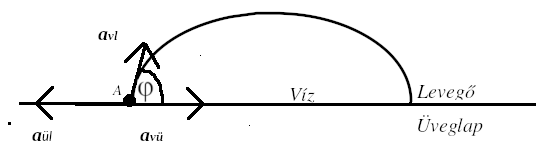
\includegraphics[width=0.7\textwidth]{tetel72.png}
		\caption{Az üveglapon lévő vízcsepp, rajta A egyensúlyban lévő ponttal és a rá ható erőkkel \label{fig:illeszkedesi_szog}}
	\end{center}
\end{figure}

\section{Görbített határfelület}

\begin{figure}[htbp]
	\begin{center}
		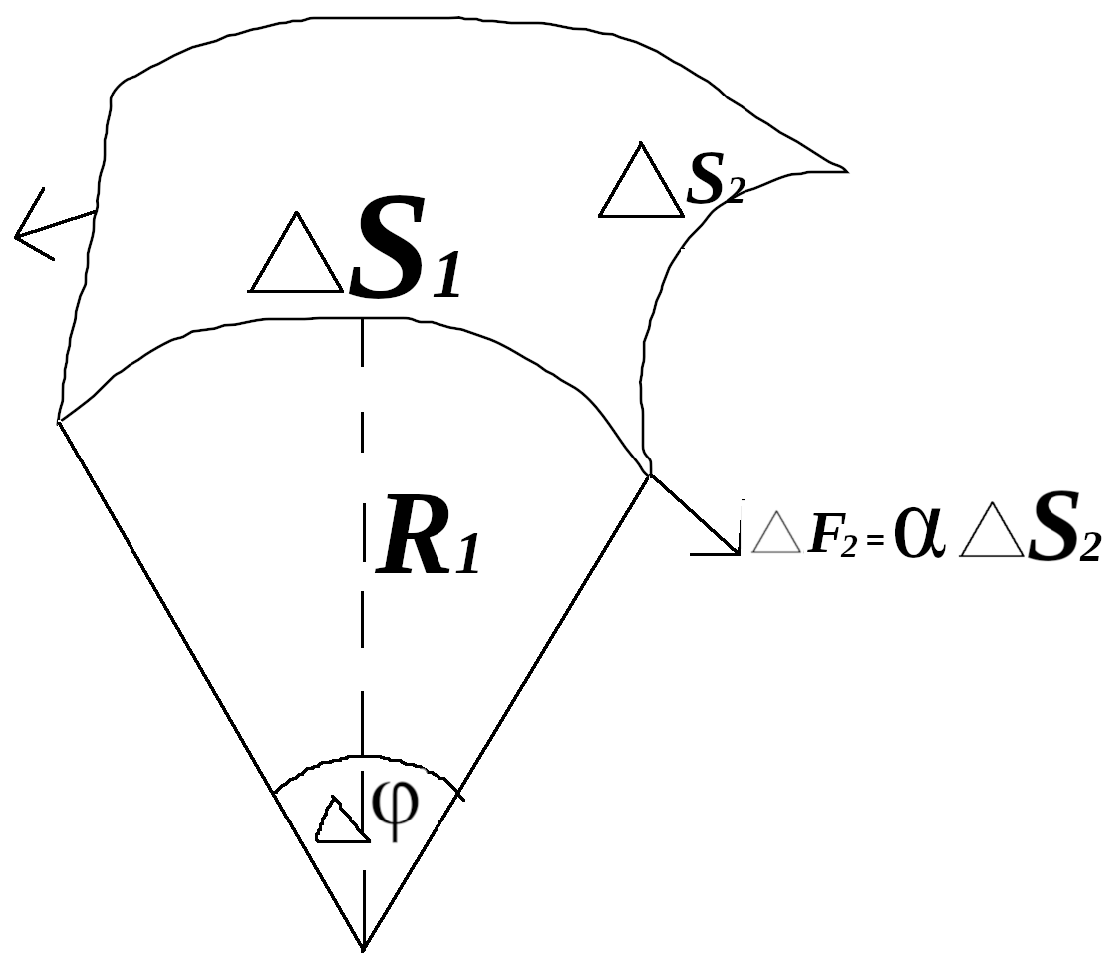
\includegraphics[width=0.4\textwidth]{tetel73.png}
		\caption{Egy kifeszített $\alpha$ felületi feszültségű görbe hártya. }
	\end{center}
\end{figure}

\noindent
A felület szélein fellépő $\Delta F_{2}$ erők függőleges komponense: $$ \Delta F_{2_{f}} =2\alpha\Delta S_{2}\cdot\sin{\frac{\Delta\varphi}{2}}=\alpha\Delta S_{2}\cdot\Delta\varphi=\alpha\Delta S_{2}\Delta S_{1} \frac{1}{R_2} $$

\noindent
Mivel a másik szélnél is lép fel erő, így a teljes függőleges erőre az alábbi képlet adódik: $$ \Delta F_{f}=\alpha(\frac{1}{R_{1}}+\frac{1}{R_{2}})\Delta S_{1}\Delta S_{2} $$

\noindent
A $\Delta F_{f}$-et kompenzálhatja a nyomáskülönbség. $$ \Delta F_{f}=p\Delta A=p\Delta S_{1}\Delta S_{2}$$

\noindent
A gömbfelületi nyomásra így a következő egyenletet kapjuk: $$p_{g}=\alpha(\frac{1}{R_{1}}+\frac{1}{R_{2}}) $$

\noindent
Ebből is látszik, hogy kisebb sugarú gömb esetén a gömbfelületi nyomás nagyobb. Szilárd anyagok esetén a nyomás helyett a feszültségtenzor használata a célszerű. A feszültségtenzor a határon ugrik.

\part*{Kapilláris emelkedés }

\begin{figure}[htbp]
	\begin{center}
		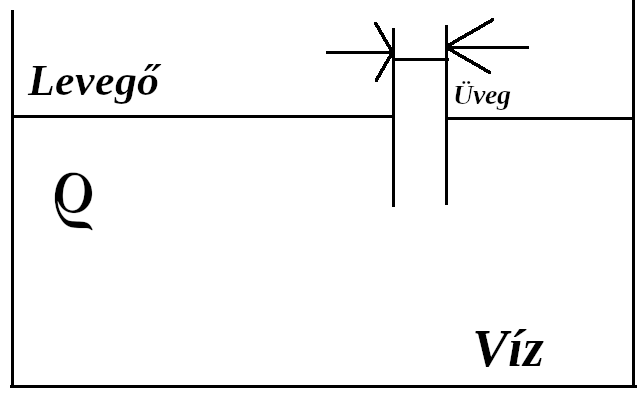
\includegraphics[width=0.3\textwidth]{tetel74.png}
		\caption{A vízbe merített kapilláris csőben a víz magasabban áll, mint az edényben.}
	\end{center}
\end{figure}

\noindent
Az emelkedés energetikai leírása: $$ W(h)=r^{2}h\varrho g \frac{h}{2}+2r\pi h\alpha_{uv}-2r\pi h\alpha_{ul}$$

\noindent
Ahol $\frac{h}{2}$ a tömegközéppont emelkedése.

\noindent
Ez akkor lesz egyensúlyban, ha a $W(h)$ függvénynek minimuma van, azaz: $$\frac{dW}{dh}=0=r^2\pi\varrho gh+(\alpha_{uv}-\alpha_{ul})2r\pi=0 $$ 

\noindent
Amit egyszerűsítve és átrendezve az alábi képletet kapjuk: $$h=\frac{2(\alpha_{ul}-\alpha_{uv})}{\varrho gr}=-\frac{\alpha_{vl}\cos{\varphi}}{\varrho gr}$$

\noindent
Ahol $\varphi$ az illeszkedési szög.

\noindent
Valójában a kialakuló folyadék felülete nem vízszintes, de ez a $\Delta h$ elhanyagolható a h-hoz képest.

\noindent
A $h$ lehet negatív is, például a higanynál.

\noindent
A képletben is látszik az, amit már tapasztalatból megfigyelhettünk, azaz hogy az emelkedés vastag csőben elhanyagolható.


\end{document}